\documentclass{article}
\usepackage{graphicx}
\usepackage[round]{natbib}
\bibliographystyle{plainnat}
\usepackage[pdfstartview=FitH,%
bookmarksnumbered=true,bookmarksopen=true,%
colorlinks=true,pdfborder=001,citecolor=blue,%
linkcolor=blue,urlcolor=blue]{hyperref}
\begin{document}
\title{Research plan under the Post-doctorate program at xx University}
%\subtitle{aa}
\author{Robert He}
\date{2008/04/23}
\maketitle
\newpage
\tableofcontents
\newpage

\section{Research Title}
~~~~Crustal seismic anisotropy in the xx using Moho P-to-S converted phases.


\section{Research Background \& Purposes}


~~~~Shear-wave splitting analyses provide us a new way to study the seismic structure and mantle dynamics in the crust and mantle. The crustal anisotropy is developed due to various reasons including lattice-preferred orientation (LPO) of mineral crystals and oriented cracks. 
\newline

Traditionally, the earthquakes occurring in the curst and the subducting plates are selected to determine the seismic anisotropy of the crust. However, none of these methods can help us to assess the anisotropy in the whole crust.  Because crustal earthquakes mostly are located in the upper crust, they do not provide information of lower crust. On the other hand, earthquakes in the subducting plates provide information of the whole crust but combined with upper mantle. However, it’s difficult to extract the sole contribution of the crust from the measurement. Fortunately P-to-S converted waves (Ps) at the Moho are ideal for investigation of crustal seismic anisotropy since they are influenced only by the medium above the Moho. Moho. Figure \ref{crustalspliting}~schematically shows the effects of shear wave splitting on Moho Ps phases. Initially, a near-vertically incident P wave generates a radially polarized converted shear wave at the crust-mantle boundary. The phases, polarized into fast and slow directions, progressively split in time as they propagate through the anisotropic media. Here, the Ps waves can be obtained from teleseismic receiver function analysis. 
%
%
\begin{figure}[htbp]
\begin{center}
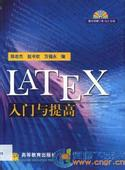
\includegraphics[width=0.47\textwidth]{crustalsplit.jpg}
\caption{The effects of shear wave splitting in the Moho P to S converted phase. Top shows a schematic seismogram in the fast/slow coordinate system with split horizontal Ps components.(cited from: McNamara and Owens, 1993)}
\label{crustalspliting}
\end{center}
\end{figure}
%
%

The Korean Peninsula is composed of three major Precambrian massifs, the Nangrim, Gyeongii, and Yeongnam massifs(Fig.\ref{geomap}). The Pyeongbuk-Gaema Massif forms the southern part of Liao-Gaema Massif of southern Manchuria, and the Gyeonggi and Mt. Sobaeksan massifs of the peninsula are correlated with the Shandong and Fujian Massifs of China. 
%
\begin{figure}[htbp]
\begin{center}
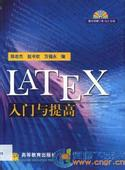
\includegraphics[width=0.755\textwidth]{crustalsplit.jpg}
\caption{Simplified geologic map. NCB: North China block; SCB: South China block.(cited from: Choi et al., 2006)}
\label{geomap}
\end{center}
\end{figure}
%

Our purpose of the study is to measure the shear wave splitting parameters in the crust of the Korean Peninsula. The shear wave splitting parameters include the splitting time of shear energy 
between the fast and slow directions, as well as fast-axis azimuthal direction in the Korean Peninsula. These two parameters provide us constraints on the mechanism causing the crustal anisotropy. From the splitting time, the layer thickness of anisotropy will be estimated. Whether crustal anisotropy mainly contributed by upper or lower crustal or both will be determined. Based on the fast-axis azimuthal direction, the tectonic relation between northeastern China and the Korean peninsula will be discussed. 


\section{Research Methods} 
   

~~~~Several methods have been introduced for calculation of receiver functions. An iterative deconvolution technique may be useful for this study since it produces more stable receiver function results than others. The foundation of the iterative deconvolution approach is a least-squares minimization of the difference between the observed horizontal seismogram and a predicted signal generated by the convolution of an iteratively updated spike train with the vertical-component seismogram. First, the vertical component is cross-correlated with the radial component to estimate the lag of the first and largest spike in the receiver function (the optimal time is that of the largest peak in the absolute sense in the cross-correlation signal). Then the convolution of the current estimate of the receiver function with the vertical-component seismogram is subtracted from the radial-component seismogram, and the procedure is repeated to estimate other spike lags and amplitudes. With each additional spike in the receiver function, the misfit between the vertical and receiver-function convolution and the radial component seismogram is reduced, and the iteration halts when the reduction in misfit with additional spikes becomes insignificant.
\newline

    For all measurement methods of shear-wave splitting, time window of waveform should be selected. Conventionally the shear-wave analysis window is picked manually. However, manual window selection is laborious and also very subjective; in many cases different windows give very different results.
\newline

    In our study, the automated S-wave splitting technique will be used, which improves the quality of shear-wave splitting measurement and removes the subjectivity in window selection. First, the splitting analysis is performed for a range of window lengths. Then a cluster analysis is applied in order to find the window range in which the measurements are stable. Once clusters of stable results are found, the measurement with the lowest error in the cluster with the lowest variance is presented for the analysis result.


\section{Expected results \& their contributions}
  

~~~~First, the teleseismic receiver functions(RFs) of all stations including radial and transverse RFs can be gained. Based on the analysis of RFs, the crustal thickness can be estimated in the Korean Peninsula. Then  most of the expected results are the shear-wave splitting parameters from RFs analysis in the crust beneath the Korean Peninsula. The thickness of anisotropic layer will be estimated in the region when the observed anisotropy is assumed from a layer of lower crustal material.All the results will help us to understand the crustal anisotropy source. 
\newline

Crustal anisotropy can be interpreted as an indicator of the crustal stress/strain regime. In addition, since SKS splitting can offer  the anisotropy information contributed by the upper mantle but combined with the crust, the sole anisotropy of the upper mantle can be attracted from the measurement of SKS splitting based on the crustal splitting result. 
 
%\cite{frogge2007}
%%
%\citep{frogge2008}
%%
%\citep{s-frogge2007}
%  5. References
\begin{thebibliography}{99}
\item Burdick, L. J. and C. A. Langston, 1977, Modeling crustal structure through the use of converted phases in teleseismic body waveforms, \textit{Bull. Seismol. Soc. Am.}, 67:677-691.

\item Cho, H-M. et al., 2006, Crustal velocity structure across the southern Korean Peninsula from seismic refraction survey, \textit{Geophy. Res. Lett.} 33, doi:10.1029/2005GL025145.

\item Cho, K. H. et al., 2007, Imaging the upper crust of the Korean peninsula by surface-wave tomography, \textit{Bull. Seismol. Soc. Am.}, 97:198-207.

\item Choi, S. et al., 2006, Tectonic relation between northeastern China and the Korean peninsula revealed by interpretation of GRACE satellite gravity data, \textit{Gondwana Research}, 9:62-67.

\item Chough, S. K. et al., 2000, Tectonic and sedimentary evolution of the Korean peninsula: a review and new view, \textit{Earth-Science Reviews}, 52:175-235.

\item Crampin, S., 1981, A review of wave motion in anisotropic and cracked elastic-medium, \textit{Wave Motion}, 3:343-391.

\item Fouch, M. J. and S. Rondenay, 2006, Seismic anisotropy beneath stable continental interiors, \textit{Phys. Earth Planet. Int.}, 158:292-320.

\item Herquel, G. et al., 1995, Anisotropy and crustal thickness of Northern-Tibet. New constraints for tectonic modeling, \textit{Geophys. Res. Lett.}, 22(14):1 925-1 928.

\item Iidaka, T. and F. Niu, 2001, Mantle and crust anisotropy in the eastern China region inferred from waveform splitting of SKS and PpSms, \textit{Earth Planets Space}, 53:159-168.

\item Kaneshima, S., 1990, Original of crustal anisotropy: Shear wave splitting studies in Japan, \textit{J. Geophys. Res.}, 95:11 121-11 133.

\item Kim, K. et al., 2007, Crustal structure of the Southern Korean Peninsula from seismic wave generated by large explosions in 2002 and 2004, \textit{Pure appl. Geophys.}, 164:97-113.

\item Kosarev, G. L. et al., 1984, Anisotropy of the mantle inferred from      observations of P to S converted waves, \textit{Geophys. J. Roy. Astron. Soc.}, 76:209-220.

\item Levin, V. and J. Park, 1997, Crustal anisotropy in the Ural Mountains foredeep from teleseismic receiver functions, \textit{Geophys. Res. Lett.}, 24(11):1 283 1286.

\item Ligorria, J. P. and C. J. Ammon, 1995, Iterative deconvolution and receiver-function estimation. \textit{Bull. Seismol. Soc. Am.}, 89:1 395-1 400.

\item Mcnamara, D. E. and T. J. Owens, 1993, Azimuthal shear wave velocity anisotropy in the basin and range province using Moho Ps converted phases, \textit{J. Geophys. Res.}, 98:12 003-12 017.

\item Peng, X. and E. D. Humphreys, 1997, Moho dip and crustal anisotropy in northwestern Nevada from teleseismic receiver functions, \textit{Bull. Seismol. Soc. Am.},  87(3):745-754.

\item Sadidkhouy, A. et al., 2006, Crustal seismic anisotropy in the south-central Alborz region using Moho Ps converted phases, \textit{J. Earth \& Space Physics}, 32(3):23-32.

\item Silver, P. G. and W. W. Chan, 1991, Shear wave splitting and subcontinental mantle deformation, \textit{J. Geophys. Res.},96:16 429-16454.

\item Teanby, N. A. et al., 2004, Automation of shear wave splitting measurement using cluster analysis, \textit{Bull. Seismol. Soc. Am.}, 94:453-463.

\item Vinnik, L. and J-P. Montagner, 1996, Shear wave splitting in the mantle Ps phases, \textit{Geophys. Res. Lett.}, 23(18):2 449- 2 452.

\item Yoo, H. J. et al., 2007, Imaging the three-dimensional crust of the Korean peninsula by joint inversion of surface-wave dispersion of teleseismic receiver functions, \textit{Bull. Seismol. Soc. Am.}, 97(3):1 002-1 011.

\item Zhu, L., and H. Kanamori, 2000, Moho depth variation in Southern California from teleseismic receiver functions, \textit{J. Geophys. Res.}, doi :10.1029/1999JB900322, 105:2 969-2 980.

\end{thebibliography}
%
%
%
%

\end{document}
